\section*{Lecture 18}

\subsection*{1.} Consider the mixing problem depicted in \textbf{\autoref{fig:f18_1}} (assuming oil and water is always well-mixed). Derive the system of equations that describe the dynamics of the amount $y_1(t)$ of oil in tank $T_1$, and the amount $y_2(t)$ of oil in tank $T_2$. Here, $t$ denotes time. (You do not need to solve the system of equations.)

\begin{figure} [ht]
  \centering
  \caption{}
  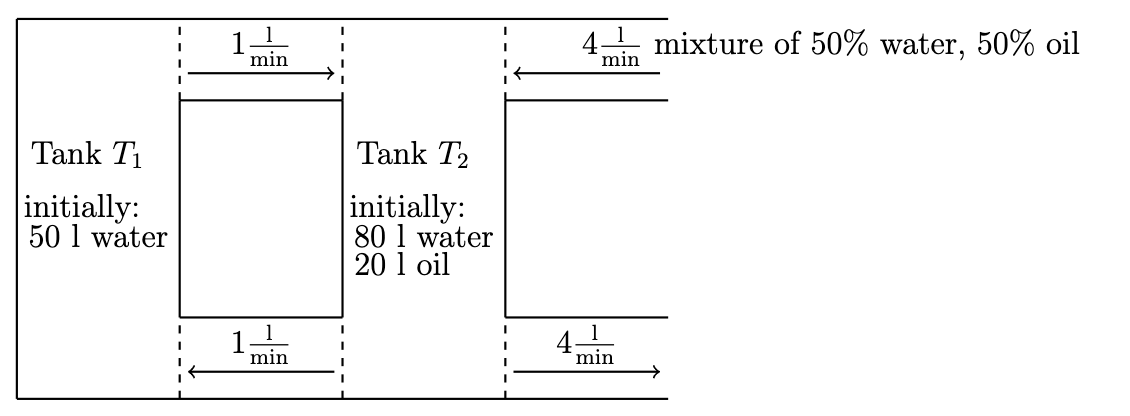
\includegraphics[width=0.75\linewidth]{../figures/f18_1.png}
  \label{fig:f18_1}
\end{figure}
\bigbreak
We denote the amount of oil in tank $T_1$ as $y_1(t)$ and vice versa for tank $T_2$. We will consider the change in the amount of oil after a small amount of time $\Delta t$ passes. This is:
\[ 
y_1(t + \Delta t) = y_1(t) + \num{0,01}y_2(t)\Delta t - \num{0,02}y_1(t)\Delta t
.\]
By subtracting $y_1(t)$ and dividing by $\Delta t$ we get:
\[ 
\frac{y_1(t + \Delta t) - y_1(t)}{\Delta t} = \num{0,01}y_2(t) - \num{0,02} y_1(t)
.\]
As $\Delta t \to 0$ we get:
\[ 
\lim_{\Delta t \to 0} \frac{y_1(t + \Delta t) - y_1(t)}{\Delta t} = y_1'(t) = \num{0,01} y_2(t) - \num{0,02} y_1(t)
.\]
The same can be done for $T_2$ which yields:
\begin{align*}
  y_2(t + \Delta t) &= y_2(t) + \num{0,02}y_1(t) \Delta t - \num{0,05}y_2(t) \Delta t + 2 \Delta t \\
  \implies y_2'(t) &= \num{0,02} y_1(t) - \num{0,05} y_2(t) + 2 \\
.\end{align*}
All in all this corresponds to the system:
\begin{align*}
  y_1'(t) &= -\num{0,02}y_1(t) + \num{0,01} y_2(t) \\
  y_2'(t) &= \num{0,02} y_1(t) - \num{0,05}y_2(t) + 2
.\end{align*}
Now we can define:
\begin{align*}
  \Vec{y}(t) &= \begin{pmatrix}
  y_1(t)\\
  y_2(t)\\
  \end{pmatrix} \\
  \Vec{y}'(t) &= \begin{pmatrix}
  y_1'(t)\\
  y_2'(t)\\
  \end{pmatrix} \\
  \Vec{g}_0 &= \begin{pmatrix}
  0\\
  2\\
  \end{pmatrix} \\
  A &= \begin{pmatrix}
  -\num{0,02}  & \num{0,01} \\
  \num{0,02}  & -\num{0,05} \\
  \end{pmatrix}
.\end{align*}
And write it as:
\[ 
\Vec{y}'(t) = A \Vec{y}(t) + \Vec{g}_0
.\]



\subsection*{2.} Solve the IVP
\[ 
\Vec{y}'(t) = A \Vec{y}(t) + \Vec{g} (t), \qquad \Vec{y}(0) = \frac{1}{3} \begin{pmatrix}
1\\
-1\\
\end{pmatrix},\qquad  A = \begin{pmatrix}
1 & -1\\
-1 & 1\\
\end{pmatrix}, \qquad \Vec{g}(t) = \begin{pmatrix}
 e^{-t}\\
 e^{t}\\
\end{pmatrix}
\]
using the method of undetermined coefficients.

\textit{Hint:} Use the sum rule.
\bigbreak
We start by finding the eigenvalues of $A$ as:
\[ 
\mathrm{det}(A - \lambda I) = \begin{pmatrix}
1 - \lambda & -1\\
-1 & 1 -\lambda\\
\end{pmatrix} = \left( 1-\lambda \right)^2 -1 = 0 \implies \lambda_1 = 0, \lambda_2 = 2
.\]
We can now find the eigenvector for $\lambda_1 = 0$ as:
\[ 
A \Vec{x}^{(1)} = \Vec{0} \implies \begin{pmatrix}
1 & -1\\
-1 & 1\\
\end{pmatrix} \begin{pmatrix}
x_1^{(1)}\\
x_2^{(1)}\\
\end{pmatrix} = \begin{pmatrix}
0\\
0\\
\end{pmatrix}
.\]
Here we choose $\Vec{x}^{(1)} = \begin{pmatrix}
1\\
1\\
\end{pmatrix}$. The same can be done for $\lambda_2 = 2$ as:
\[ 
  (A-2I) \Vec{x}^{(2)} = \Vec{0} \implies \begin{pmatrix}
  -1 & -1\\
  -1 & -1\\
  \end{pmatrix} \begin{pmatrix}
  x_1^{(2)}\\
  x_2^{(2)}\\
  \end{pmatrix} = \begin{pmatrix}
  0\\
  0\\
  \end{pmatrix}
.\]
Here we choose $\Vec{x}^{(2)} = \begin{pmatrix}
1\\
-1\\
\end{pmatrix}$. The general solution of the corresponding homogeneous ODE is therefore:
\[ 
\Vec{y}_h(t) = c_1 \Vec{x}^{(1)} e^{\lambda_1 t} + c_2 \Vec{x}^{(2)} e^{\lambda_2 t} = c_1 \begin{pmatrix}
1\\
1\\
\end{pmatrix} + c_2 \begin{pmatrix}
1\\
-1\\
\end{pmatrix} e^{2t}
.\]
We can rewrite the nongomogeneous term as:
\[ 
\Vec{g}(t) = \begin{pmatrix}
1\\
0\\
\end{pmatrix} e^{-t} + \begin{pmatrix}
0\\
1\\
\end{pmatrix} e^{t}
.\]
The basic and sum rules therefore gives:
\[ 
\Vec{y}_r(t) = \Vec{u} e^{-t} + \Vec{v} e^{t}, \Vec{u} = \begin{pmatrix}
u_1\\
u_2\\
\end{pmatrix}, \Vec{v} = \begin{pmatrix}
v_1\\
v_2\\
\end{pmatrix}
.\]
We can now insert this into the nonhomogeneous system as:
\[ 
\Vec{y}_r'(t) = A \Vec{y}_r(t) \implies - \Vec{u} e^{-t} + \Vec{v} e^{t} = e^{-t} A \Vec{u} + e^{t} A \Vec{v} + e^{-t} \begin{pmatrix}
1\\
0\\
\end{pmatrix} + e^{t} \begin{pmatrix}
0\\
1\\
\end{pmatrix}
.\]
By comparing terms of the same type we can see that:
\begin{align*}
  - \Vec{u} &= A \Vec{u} + \begin{pmatrix}
  1\\
  0\\
  \end{pmatrix} \\
    \Vec{v} &= A \Vec{v} + \begin{pmatrix}
    0\\
    1\\
    \end{pmatrix}
.\end{align*}
This can also be written as:
\begin{align*}
  -u_1 &= u_1 - u_2 + 1  \\
  -u_2 &= -u_1 + u_2 \\
  v_1 &= v_1 - v_2 \\
  v_2 &= -v_1 + v_2 + 1 \\
  \implies u_1 &= -\frac{2}{3}, u_2 = -\frac{1}{3}, v_1 = 1, v_2 = 0 \\
.\end{align*}
This gives the nonhomogeneous solution:
\[ 
\Vec{y}_r(t) = \begin{pmatrix}
-\frac{2}{3}\\
-\frac{1}{3}\\
\end{pmatrix} e^{-t} + \begin{pmatrix}
1\\
0\\
\end{pmatrix} e^{t}
.\]
The general solution of the nonhomogeneous system is therefore:
\[ 
\Vec{y}(t) = \Vec{y}_h(t) + \Vec{y}_r(t) = c_1 \begin{pmatrix}
1\\
1\\
\end{pmatrix} + c_2 \begin{pmatrix}
1\\
-1\\
\end{pmatrix} e^{2t} + \begin{pmatrix}
-\frac{2}{3}\\
-\frac{1}{3}\\
\end{pmatrix} e^{-t} + \begin{pmatrix}
1\\
0\\
\end{pmatrix} e^{t}
.\]
We can now introduce the initial condition as:
\begin{align*}
  c_1 \begin{pmatrix}
  1\\
  1\\
  \end{pmatrix} + c_2 \begin{pmatrix}
  1\\
  -1\\
  \end{pmatrix} + \begin{pmatrix}
  -\frac{2}{3}\\
  -\frac{1}{3}\\
  \end{pmatrix} + \begin{pmatrix}
  1\\
  0\\
  \end{pmatrix} = \frac{1}{3} \begin{pmatrix}
  1\\
  -1\\
  \end{pmatrix}
.\end{align*}
From this we get:
\begin{align*}
  c_1 + c_2 &= 0 \\
  c_1 - c_2 &= 0
.\end{align*}
Which means $c_1 = c_2 = 0$. Therefore the particular solution is:
\[ 
\Vec{y}_p(t) = y_r(t) = \begin{pmatrix}
-\frac{2}{3}\\
-\frac{1}{3}\\
\end{pmatrix} e^{-t} + \begin{pmatrix}
1\\
0\\
\end{pmatrix}e^{t}
.\]



\subsection*{3.} Find the general solution of
\[ 
\Vec{y}'(t) = A \Vec{y}(t) + \Vec{g}(t), A = \begin{pmatrix}
1 & -1\\
-1 & 1\\
\end{pmatrix}, \Vec{g}(t) = \begin{pmatrix}
 e^{2t}\\
- e^{2t}\\
\end{pmatrix}
\]
using the method of undetermined coefficients.
\bigbreak
We have already found the solution to the corresponding homogeneous equation in Exercise 2:
\[ 
\Vec{y}_h(t) = c_1 \begin{pmatrix}
1\\
1\\
\end{pmatrix} + c_2 \begin{pmatrix}
1\\
-1\\
\end{pmatrix} e^{2t}
.\]
From the basic rule we have that:
\[ 
\Vec{g}(t) = e^{2t} \begin{pmatrix}
1\\
-1\\
\end{pmatrix} \implies \Vec{y}_r(t) = \Vec{v}e^{2t}, \quad \Vec{v} = \begin{pmatrix}
v_1\\
v_2\\
\end{pmatrix}
.\]
Since $e^{2t}$ is a term in both $\Vec{y}_h$ and $\Vec{y}_r$ we must use the modification rule. This gives:
\[ 
\Vec{y}_r(t) = \Vec{u} t e^{2t} + \Vec{v} e^{2t}, \quad \Vec{u} = \begin{pmatrix}
u_1\\
u_2\\
\end{pmatrix}, \quad \Vec{v} = \begin{pmatrix}
v_1\\
v_2\\
\end{pmatrix}
.\]
We can now find the derivative of this so we can insert it into the nonhomogeneous system as:
\[ 
\Vec{y}'_r(t) = \Vec{u} e^{2t} + 2 \Vec{u} t e^{2t} + 2 \Vec{v} e^{2t}
.\]

We now insert this into the nonhomogeneous system as:
\[ 
\Vec{y}'_r (t) = A \Vec{y}(t) + \Vec{g}(t) \implies \Vec{u} e^{2t} + 2 \Vec{u} t e^{2t} + 2 \Vec{v} e^{2t} = t e^{2t} A \Vec{u} + e^{2t} A \Vec{v}  + e^{2t} \begin{pmatrix}
1\\
-1\\
\end{pmatrix}
.\]
We can now compare terms of the same type (i.e., $e^{2t}$ and $te^{2t}$) as:
\begin{align*}
  \Vec{u} + 2 \Vec{v} &= A \Vec{v} + \begin{pmatrix}
  1\\
  -1\\
  \end{pmatrix}\\
  2 \Vec{u} &= A \Vec{u}
.\end{align*}
From this we see that $\Vec{u}$ is the eigenvector of $A$ corresponding to the eigenvalue 2. This was found in Exercise 2 to e:
\[ 
\Vec{u} = c\begin{pmatrix}
1\\
-1\\
\end{pmatrix}, \quad c \neq 0
.\]
We can now insert this into the first expression from above as:
\begin{align*}
  c + 2 v_1 &= v_1 - v_2 + 1\\
  -c + 2 v_2 &= - v_1 + v_2 -1 \\
  \implies - v_1 - v_2 &= c - 1 \\
  -v_1 - v_2 &= -c + 1 \\
  \implies c &= 1,
.\end{align*}
Now we can choose $v_1 = v_2 = 0$. Therefore the nonhomogeneous solution is:
\[ 
\Vec{y}_r(t) = \begin{pmatrix}
1\\
-1\\
\end{pmatrix} t e^{2t}
.\]
The general solution therefore is:
\[ 
\Vec{y}(t) = \Vec{y}_h(t) + \Vec{y}_r(t) = c_1 \begin{pmatrix}
1\\
1\\
\end{pmatrix} + c_2 \begin{pmatrix}
1\\
-1\\
\end{pmatrix} e^{2t} + \begin{pmatrix}
1\\
-1\\
\end{pmatrix} te^{2t}
.\]



\subsection*{4.} Find the general solution of
\[ 
\Vec{y}'(t) = A \Vec{y}(t) + \Vec{g}(t), A = \begin{pmatrix}
1 & -1\\
-1 & 1\\
\end{pmatrix}, \Vec{g}(t) = \begin{pmatrix}
 e^{2t}\\
 -e^{2t}\\
\end{pmatrix}
\]
using the method of variation of parameters.
\bigbreak
From Exercise 2 we have the general solution to the corresponding homogeneous ODE. This is:
\[ 
\Vec{y}_h(t) = c_1 \begin{pmatrix}
1\\
1\\
\end{pmatrix} + c_2 \begin{pmatrix}
1\\
-1\\
\end{pmatrix} e^{2t}
.\]
From variation of parameters we have:
\[ 
\Vec{y}_r(t) = u_1(t) \begin{pmatrix}
1\\
1\\
\end{pmatrix} + u_2(t) \begin{pmatrix}
1\\
-1\\
\end{pmatrix} e^{2t}
.\]
We now insert this into the nonhomogeneous system as:
\begin{align*}
  \Vec{y}'_r(t) &= A \Vec{y}_r(t) + \Vec{g}(t) \\
  \implies u_1'(t) \begin{pmatrix}
  1\\
  1\\
  \end{pmatrix} + u'_2(t) \begin{pmatrix}
  1\\
  -1\\
  \end{pmatrix} e^{2t} + 2 u_2(t) \begin{pmatrix}
  1\\
  -1\\
  \end{pmatrix} e^{2t} &= u_2 (t) e^{2t} \begin{pmatrix}
  2\\
  -2\\
  \end{pmatrix} + e^{2t} \begin{pmatrix}
  1\\
  -1\\
  \end{pmatrix} \\
  \implies u_1'(t) \begin{pmatrix}
  1\\
  1\\
  \end{pmatrix} + u'_2(t) \begin{pmatrix}
  1\\
  -1\\
  \end{pmatrix} e^{2t} &= e^{2t} \begin{pmatrix}
  1\\
  -1\\
  \end{pmatrix}
.\end{align*}
Which can be written in components as:
\begin{align*}
  u_1'(t) + u_2'(t) e^{2t} &= e^{2t} \\
  u_1'(t) - u_2'(t) e^{2t} &= - e^{2t}
.\end{align*}
From this we can quickly see that $u_1'(t) = 0 \implies u_1(t) = \mathrm{const.} = a$. We also see that $u_2'(t) = 1 \implies u_2(t) = t + b, b = \mathrm{const.}$. If we choose $a = 0$ and $b = 0$ we get:
\[ 
\Vec{y}_r(t) = \begin{pmatrix}
1\\
-1\\
\end{pmatrix} t e^{2t}
.\]
The general solution to the system of equations is therefore:
\[ 
\Vec{y}(t) = \Vec{y}_h(t) + \Vec{y}_r(t) = c_1 \begin{pmatrix}
1\\
1\\
\end{pmatrix} + c_2 \begin{pmatrix}
1\\
-1\\
\end{pmatrix} e^{2t} + \begin{pmatrix}
1\\
-1\\
\end{pmatrix} t e^{2t}
.\]





